\documentclass[review]{elsarticle}
\input{packages.tex}

\begin{document}
\begin{frontmatter}

\title{Disclosing the heat density of \replaced{district heating}{centralized heat} networks \replaced{for}{in} Austria \added{in} 2050 under the \added{remaining European CO\textsubscript{2} budget of the} 1.5°C climate target}

\author[1,2]{Sebastian Zwickl-Bernhard\corref{cor1}}
\ead{zwickl@eeg.tuwien.ac.at}
\author[2]{Daniel Huppmann}
\author[1]{Antonia Golab}
\author[1]{Hans Auer}
\cortext[cor1]{Corresponding author}
\address[1]{Energy Economics Group (EEG), Technische Universität Wien, Gusshausstrasse 25-29/E370-3, 1040 Wien, Austria}
\address[2]{Energy, Climate and Environment (ECE) Program,  International Institute for Applied Systems Analysis (IIASA), Laxenburg, Austria}

\begin{abstract}
	\added{We downscale the cost-effective heat supply of different European decarbonization scenarios generated by the aggregate model GENeSYS-MOD from the national to the community level in Austria. The remaining European CO\textsubscript{2} budget (and related CO\textsubscript{2} prices) of the 1.5°C climate target is considered in the values to be downscaled. The results show, among others, that district heating covers parts of the heat demand in four of the thirty-five sub-regions in Austria in 2050. The district heating networks are located in densely populated areas with high heat demands and are supplied by geothermal, synthetic gas, hydrogen, and waste. Not all of these networks reach the heat density required for economic and technical efficiency from today’s techno-economic perspective and industry benchmarks. The identified heat density gap, mainly driven by lower heat demands, can be reduced and even closed by an optimal allocation of large-scale heat pump generation into district heating. We conclude that district heating networks still reach economic viability in 2050.}
\end{abstract}

\begin{keyword}
	District heating, heat density, \added{network topology}, 1.5°C climate target, downscaling, 2050
\end{keyword}
\end{frontmatter}

\section*{Nomenclature}
\begin{center}
	\renewcommand{\arraystretch}{1.1}
	\centering
	\small
	\begin{tabular}{lm{8cm}r}
		Type & Description & Unit\\
		\hline
		Set and index & & \\
		\hline
		{$t \in \mathcal{T}=\{1,\ldots,T\}$} & Set of heat sources/generation technologies, index by $t$\\
		{$r \in \mathcal{R}=\{1,\ldots,R\}$} & Set of sub-regions, index by $r$\\
		{$s \in \mathcal{S}=\{0,1,*\}$} & Stage of iterations, index by $s$\\
		\hline
		Variables\\
		\hline
		{$q_{t}$} & Heat generation per $t$ & \SI{}{TWh}\\
		{$\rho_{r}$} & Population density per $r$ & \SI{}{1 \per \per km^2}\\
		{$p_{r}$} & Total population per $r$ & \SI{}{1}\\
		{$\sigma_{t}$} & Minimal network infrastructure requirements per $t$& \SI{}{1 \per \per km^2}\\
		{$\pi_{r}$} & Available potential of network infrastructure per $r$& \SI{}{1 \per \per km^2}\\
		{$\hat{q}_{t,r}$} & Heat generation per $t$ and $r$& \SI{}{TWh}\\
		{$q^{heat}_{r}$} & Heat demand per $r$& \SI{}{TWh}\\
		{$\tilde{q}_{t}$} & Available heat generation per $t$& \SI{}{TWh}\\
		{$G^{s}$} & District heating network graph at $s$ & \\
		{$n^{s}$} & Node of district heating network graph at $s$ & \\
		{$l^{s}_{k,j}$} & Line connecting nodes $k$ and $j$ at $s$ & \\
		{$q^{s}_{n^{s}}$} & Nodal district heating at $s$ & \SI{}{TWh}\\
		{$\tilde{q}^{s}_{n^{s}}$} & Nodal on-site heat generation at $s$ & \SI{}{TWh}\\
		{$\pi^{s}_{n^{s}}$} & Nodal benchmark indicator value at $s$ & \SI{}{1}\\
		{$\alpha_{n^{s}}$} & Number of triangles with direct neighboring nodes & \SI{}{1}\\
		{$\beta_{n^{s}}$} & Number of connection lines to the graph & \SI{}{1}\\		
		\hline
	\end{tabular}
\end{center}
\newpage

% although substantial heat saving measures are installed
\section{Introduction}
The Paris Climate Agreement sets the global framework for mitigating climate change \cite{agreement2015paris}. It stipulates that the increase in the global average temperature should be kept well below \SI{2}{\degreeCelsius} compared to 1990. In addition, further measures are developed, aiming at a maximum increase of \SI{1.5}{\degreeCelsius}. However, it is also about humanity adapting to the negative effects of climate change that are already being felt. The IPCC Special Report on \SI{1.5}{\degreeCelsius} (SR1.5) summarizes the state of scientific knowledge globally on the consequences of global warming \cite{edenhofer2011ipcc}.

\subsection{Long-term global sustainable transformation plans of energy systems}
To implement the Paris Climate Agreement and the SR1.5, the European Commission has set deep decarbonization targets together with national governments. In particular, the "EU Green Deal" describes the concrete goals in Europe, namely a climate-neutral and resource-conserving economy and society (see, e.g., in \cite{kemfert2019green}). The overarching goal is emissions neutrality 2050. To achieve this long-term ambition, the European Commission recently presented "Fit for 55", a concrete roadmap to 2030. This program commits to a \SI{55}{\%} reduction in CO\textsubscript{2} emissions in 2030 compared to 1990 \cite{european_commission_european_2019}. The concrete measures affect almost all sectors of the energy system and should lead to a significant efficiency improvement and a massive overall reduction in fossil fuels. It implies, among others, binding annual targets for reducing energy consumption and an extension of the already established EU emissions trading system (EU ETS) to new sectors. In addition to transportation, the building sector will also be part of the EU ETS in the future. A separate new emissions trading system for fuel supply in these sectors will be introduced. In the buildings sector, through the annual anchored emissions reduction, this means a defined roadmap to complete decarbonization of heating and cooling demand, as the two reasons for emissions in this sector. In this paper, we look at what deep decarbonization of building heating demand may look like in 2050 in Austria and the implications of the corresponding sustainable energy mix for centralized heating networks.

\subsection{Implications and effects of the decarbonization on the heating sector}
The scope of changes required by 2030/2050 in the heating sector become even clearer at the national level. In Europe, the average share of renewable energies in the heating and cooling sector 2018 is only just above \SI{20}{\%} on average for all EU member states \cite{eurostat_reference}. It is in fact higher in some countries, for example in Austria, where it is above \SI{34}{\%}. However, fossil fuels continue to dominate there as well. To be even more specific for the heating sector: of the nearly 4,000,000 residential dwellings in Austria, more than 900,000 are heated with natural gas, and more than 500,000 with oil \cite{statistik_austria}. If these heating systems are converted to renewable energy supply by 2050, this corresponds to a retrofitting of 50,000 units per year, or more than 130 per day - only in Austria. To achieve this goal makes measures necessary that go beyond the electrification of heat and leads to an expansion of district heating networks \cite{jalil2018spatially}.\vspace{0.3cm}

Centralized heating networks are particularly advantageous for supplying densely populated or urban areas resulting from high heat densities there \cite{inage2020development}. In addition to heat density, the connection rate is a key factor determining the efficiency of district heating/cooling networks and thus their implementation. For example, currently in Austria, at a connection rate of \SI{90}{\%}, \SI{10}{GWh \per km^2} is used as a benchmark for supplying an area with district heating\footnote{\url{http://www.austrian-heatmap.gv.at/ergebnisse/}}. The reference value of \SI{10}{GWh \per km^2} is in line with findings regarding district heating networks also from the Scandinavian region (Denmark, Sweden, and Finland) \cite{zinko2008district}. These are rough estimates, but they do allow an initial assessment of the economic viability or feasibility of a district heating network. In a detailed consideration and evaluation of district heating networks numerous factors play a decisive role. Nussbaumer and Thalmann \cite{nussbaumer2016influence} thoroughly elaborate on the network design and its impact on the profitability of centralized heat networks. Laasasenaho et al. \cite{laasasenaho2019gis} emphasize in their study the optimal location of heat generation units/sources within centralized heat networks enabling a cost-optimized heat supply. Gopalakrishnan and Kosanovic \cite{gopalakrishnan2014economic} focus in their study on the optimal heat generation technology dispatch. When examining the economic viability of district heating networks, building renovation measures must also be taken into account (see, e.g., in \cite{andric2018impact} and \cite{rabani2021achieving}). Hietaharju et al. \cite{hietaharju2021stochastic} recently show in their analysis that a $2-3$\SI{}{\%} building renovation rate per year results in a decrease of $19-28$\SI{}{\%} of the long-term district heating demand. This reduces also the heat density. However, studies show that a reduction in heat density is not necessarily a barrier to district heating networks \cite{persson2011heat}. Reidhav and Werner \cite{reidhav2008profitability} show in their study how energy taxes can improve the profitability of sparse district heating networks in Sweden. Following these considerations and in light of ambitious CO\textsubscript{2} reduction targets, it can also be assumed that the rising CO\textsubscript{2} price can have a similar effect as the energy tax. Of course, this is only valid in case of deep decarbonization of the generation mix feeding into centralized heat networks. Di Lucia and Ericsson \cite{di2014low} show that biomass significantly contributed to the decarbonization of the district heating network and replaced fossil fuels in the feed-in generation mix in Sweden. Ghafghazi et al. \cite{ghafghazi2010multicriteria} also identify in their mutli-criteria study wood pellets as the optimal system options for fueling district heating networks. Eventually, also the increasing cooling demand and the co-design of centralized networks for heating and cooling can increase the economic viability of these and counteract the reduction of heat density from an economic point of view \cite{zhang2021economic}.

\subsection{Lack in the implementation of decarbonization in different sectors}
However, the concrete implementation to achieve predefined climate change mitigation goals still is lacking in many cases. For this reason, numerous studies go beyond and show roadmaps for the rapid decarbonization. For example, Rockstr{\"o}m et al. \cite{rockstrom2017roadmap} conduct such a study and propose pathways for halving gross anthropogenic CO\textsubscript{2} emissions every decade. Other works go into more depth regarding optimal solutions for the decarbonization of individual energy services. There are relevant differences between the individual sectors of the energy system related to decarbonization. How a sustainable energy service can be provided in the different sectors must therefore be examined in detail. This perspective is supported by a large number of detailed decarbonization studies covering specific energy service needs (e.g., for the building sector Leibowicz et al. \cite{leibowicz2018optimal}, transport sector Pan et al. \cite{pan2018decarbonization}, and industries Habert et al. \cite{habert2020environmental}).\vspace{0.3cm}

Despite all the details associated with the sector-specific decarbonization strategies, the principles of a net-zero society base on three key points: (i) reduction of the energy demand (see, e.g., Oshiro et al. \cite{oshiro2021enabling} and Grubler et al. \cite{grubler2018low}), (ii) deployment and generation of renewable energy technologies (see, e.g., Bakhtavar et al. \cite{bakhtavar2020assessment} focusing on net-zero districts by deployment of renewable energy generation), and (iii) increase in efficiency regarding the provision of energy services and the associated optimal utilization of sustainable energy sources. The third point (iii) includes, among others, two main aspects, namely: on the one hand, that potentials of renewable resources are exploited locally and, on the other hand, that energy carriers with various fields of application are utilized with the highest possible efficiency. We like to refer to just a few selected references without claiming to be exhaustive and focus here on hydrogen as one example of an energy carrier with high potentials in sustainable energy systems and a significant bandwidth of efficiency in terms of its generation, storage and use. Van Ruijven et al. \cite{van2007potential} highlight that the introduction of hydrogen in global energy systems only leads to lower emissions with high end-use efficiency and low-carbon production. Van Ressen \cite{van2020hydrogen} systematically investigates the possibilities and challenges of hydrogen and discusses extensively its role in the energy transition. Recently, Böhm et al. \cite{bohm2021power} comprehensively elaborate on hydrogen-related synergies and its role in sustainable heat supply.\vspace{0.3cm}

\subsection{Implications of large-scale numerical model results on the local level}
In many cases when it comes to the question of optimal solutions, researcher use numerical models. In general, these models strike a balance between complexity and aggregation. Integrated assessment models (IAMs) are large numerical models covering complex interrelations between climate, society, economics, policy, and technology. Dowlatabadi \cite{dowlatabadi1995integrated} provided 1995 a fundamental review on IAMs focusing on their role in the context of climate change. Krey et al. \cite{krey2019looking} discuss and systematically compare different IAMs. Harmsen et al. \cite{harmsen2021integrated} elaborates on the modeling behaviour of IAMs. Wilkerson et al. \cite{wilkerson2015comparison} and van Vuuren et al. \cite{van2016carbon} deal with IAMs and their role in understanding global energy decarbonization pathways. In particular, both studies examine CO\textsubscript{2} budget and price developments. Schwanitz \cite{schwanitz2013evaluating} evaluates IAMs of global climate change and discusses, among others, the appropriate level of regional (spatial) aggregation of countries in the modeling analysis. Generalizing this aspect reveals an aspect already known but essential in the context of large numerical models. It becomes necessary for modelers to set priorities regarding the level of detail, which inevitably creates trade-offs in the analysis regarding the granularity of the temporal, spatial, and other dimensions \cite{gargiulo2013long}. Gambhir et al. \cite{gambhir2019review} also highlight this aspect of aggregation bias in their critical review of IAMs. They propose, among others, that IAMs should be increasingly be supplemented with other models and analytical approaches. Not least for this reason, (large) energy models also play a significant role in the analysis of energy systems in the context of climate change. Compared to IAMs, they more strongly emphasize the level of detail in terms of techno-economic characteristics (see the review of modeling tools of energy systems in \cite{ringkjob2018review}). However, the lack of granularity remains, that these (global) energy models consider only a highly aggregated spatial resolution. To name just two selected approaches, Capros et al. \cite{capros2012model} (PRIMES) and Löffler et al. \cite{loffler2017designing} (GENeSYS-MOD) provide energy system models focusing on the European energy system with a spatial resolution on the country level. Further approaches are needed to disaggregate results obtained at the country level to finer scales, such as districts, neighborhoods, and other local levels. In this context, Backe et al. \cite{backe2021heat} provided a novel approach in the context of merging local activities/behavior in sustainable local communities into a large energy system model (bottom-up linkage). In their study, they integrated local flexibility options into the global energy system model EMPIRE, which provides in principle only country-level resolution. This and other work confirms the emerging trend of making top-down and bottom-up linkages between different spatial-temporal levels of resolution to drive decarbonization across all sectors.\vspace{0.3cm}

\subsection{Objective and contribution of this work}
Against this background, the core objective of this work is downscaling European decarbonization scenarios of the heating sector to the community/distribution grid level serving end-users in 2050. In particular, downscaling considers the highly efficient and local use of sustainable heat sources in centralized heat networks (e.g., co-firing hydrogen in cogeneration plants and large-scale waste utilization, etc.). In addition, the topography of district heating networks is of particular importance and plays a crucial role in applied downscaling. This allows estimates of realistic decarbonized district heating networks in 2050 to be obtained, which can be compared with existing networks. Thereby, the heat density of district heating networks serves as a comparative indicator and permits a rough estimation of the changes needed of centralized heating networks considering the 1.5°C climate target. An Austrian case study is conducted, downscaling the results of the heating sector in 2050 from the large numerical energy system model GENeSYS-MOD, from the country to community/distribution grid level.\vspace{0.3cm}

The method applied consists of three different scenario-independent downscaling techniques. As the first, proportional downscaling using population as proxy is used as reference (Section \ref{pop}). As the second, an sequential downscaling approach is presented, dissaggregating from the country level to the sub-region level. Thereby, population density and the infrastructure requirements of heat technologies serve as additional criterion in the downscaling (Section \ref{alg1}). And finally, an iterative downscaling algorithm is presented. The algorithm is based on graph-theory benchmarking and projects centralized heat supply on the local (community) level (Section \ref{alg2}). Section \ref{results} presents and discusses the results of this work. Section \ref{res:1} and \ref{res:2} show heat generation by source on different spatial levels. Section \ref{res:3} and \ref{res:4} present centralized heat networks on a high spatial granularity. Section \ref{res:5} synthesizes the results of centralized heat networks and compares heat densities of centralized heat networks in 2050 with today's values. Section \ref{conclusions} concludes this work and provides an outlook for future work. 
\section{Materials and methods}\label{methodology}
This section explains the methodology developed in this work. First, section \ref{res:1} presents the output from the European Horizon 2020 project openENTRANCE (incl. GENeSYS-MOD results), since this is the main input for the downscaling. Therein, information about the different heat sources/generation technologies that are downscaled is provided. \added{Section \ref{sec:eq} explains the mathematical formulation of the optimization model in detail. Then, section \ref{sec:workflow} shows the workflow that is used to determine the implemented shares of district heating.} Finally, section \ref{open} concludes this section and presents further data and open-source tools used in this work.

\subsection{Heat supply of the Austrian residential and commercial sector in 2050: four different decarbonization scenarios}\label{res:1}
This section presents the heat generation mix covering the Austrian residential and commercial heat demand in 2050 for four different scenarios, which have been developed within the European Horizon 2020 openENTRANCE project. They are named as follows: \textit{Directed Transition}, \textit{Societal Commitment}, \textit{Techno-Friendly}, and \textit{Gradual Development}. Within each of them, specific fundamental development of the energy systems is described while aiming for a sustainable transition of the provision of energy services. The first three scenarios assume different approaches to limit global warming to around \SI{1.5}{\degreeCelsius} as laid out in the Paris Agreement. Particularly, the results of these scenarios implicitly consider the remaining European fraction of the CO\textsubscript{2} budget of the 1.5°C climate target. The last scenario (\textit{Gradual Development}) can be interpreted as a less ambitious scenario, limiting global warming to around \SI{2.0}{\degreeCelsius} climate target. Accordingly, the results of this scenario consider the remaining European fraction of the CO\textsubscript{2} budget of the 2.0°C climate target. Below, the scenarios are described briefly, before the quantitative results at the country level are presented. For a more detailed description of the scenarios, refer to \cite{auer2020quantitative, auer2020development, hainsch2022energy}. Further information is also available on the website of the project\footnote{\url{https://openentrance.eu/}} and on GitHub\footnote{\url{https://github.com/openENTRANCE}}.\vspace{0.3cm}

The underlying concept of the four scenarios is a three-dimensional space consisting of the following parameters: technology, policy, and society. Each scenario describes a specific pathway to reach a decarbonized energy system taking into account a pronounced contribution of two dimensions. Regarding the third dimension, a development is assumed that leads to no significant contribution to the decarbonization of the energy system. 

\begin{itemize}
	\item \textit{Directed Transition} looks at a sustainable provision of energy services through strong policy incentives. This bundle of actions becomes necessary because neither the markets nor the society adequately pushes sustainable energy technologies.
	\item \textit{Societal Commitment} achieves deep decarbonization of the energy system by a strong societal acceptance of the sustainable energy transition and shifts in energy demand patterns. Thereby, decentralized renewable energy technologies together with policy incentives facilitate a sustainable satisfaction of energy service needs. Due to the shift in energy demand, no fundamental breakthroughs of new clean technologies are required.
	\item \textit{Techno-Friendly} describes a development of the energy system where a significant market-driven breakthrough of renewable energy technologies gives rise to the decarbonization of energy service supply. Additionally, society acceptance supports the penetration of clean energy technologies and the sustainable transition.
	\item \textit{Gradual Development} differs from the other scenarios; it assumes emissions reductions that (only) stabilize the global temperature increase at \SI{2.0}{\degreeCelsius}. At the same time, a combination of each possible sustainable development initiative of the energy system is realized in this scenario. Although the other three dimensions contribute to decarbonization, they do not push it sufficiently, and this results in a more conservative scenario than the others.
\end{itemize}

Table \ref{tab:comparison} shows the heat generation by source/technology in Austria in 2050 for the four scenarios. These values were obtained during the course of the openENTRANCE project and are generated by the open-source aggregate model GENeSYS-MOD \cite{burandt2018genesys}. 

\definecolor{Gray}{gray}{0.95}
\begin{table}[h]
	\centering
	\resizebox{1\textwidth}{!}{% use resizebox with textwidth
		\renewcommand{\arraystretch}{1.35}
		\begin{tabular}{lrrrrr}
			\toprule 
			& \multicolumn{5}{c}{obtained from GENeSYS-MOD}\\\cmidrule(lr){2-6}
			& 2020 & \multicolumn{4}{c}{2050}\\
			\cmidrule(lr){2-2}\cmidrule(lr){3-6}
			Generation by source in TWh  & - & DT & SC & TF & GD\\\hline
			Biomass & 13.00 & 3.37 & 3.37  & 3.37  & 3.37 \\
			Direct electric & 4.10 & 2.13  & 1.98 & 1.53  & 1.81 \\
			Geothermal & 0 & 2  & 2  & 2  & 2 \\
			Natural gas (fossil) & 43.67 & 0  & 0  & 0  & 0 \\
			Heat pump (air) & 11.37 & 22.73  & 15.71  & 25.96  & 9.68 \\
			Heat pump (ground) & 0 & 17.50  & 19.47  & 4.69  & 19.21 \\
			Hydrogen & 0 & 1.03  & 2.18  & 7.43  & 8.65 \\
			Oil & 0.66 & 0  & 0  & 0  & 0 \\
			Synthetic gas & 0 & 0.36  & 1.35  & 2.79  & 5.35 \\
			Waste & 1.2 & 2  & 2  & 2  & 2 \\\hline
			\cellcolor{Gray}Total & \cellcolor{Gray}74.0 &\cellcolor{Gray}51.12 & \cellcolor{Gray}48.06&\cellcolor{Gray}49.77 & \cellcolor{Gray}52.07\\
			Rel. reduction compared to 2020& - & -31\% & -35\% & -33\% & -30\%\\\hline
			District heating ($Q^{dh}_{GENe}$ in Sec. \ref{sec:eq})&  & 16.75 & 15.38 & 27.20 & 22.84\\
			\bottomrule
	\end{tabular}}
	\caption{Heat generation by source in Austria in 2020 and the four different decarbonization scenarios in 2050 \added{obtained from GENeSYS-MOD}. Geothermal, hydrogen, synthetic gas, waste, and half of heat pump (air-sourced) generation is used in district heating. Sources: \cite{auer2020development, konighofer2014potenzial, buchele2015bewertung}}
	\label{tab:comparison}
\end{table}

In this work, the naming convention of heat sources/generation technologies from GENeSYS-MOD is essentially followed to ensure consistency between aggregated (i.e., downscaling input values) and local (i.e., dowmscaling output values) levels. Nevertheless, we introduced the heat sources waste and geothermal that were initially not included in the list of heat sources from openENTRANCE results. We separated waste as part of biomass and geothermal from heat pump (ground-sourced) heat generation using estimates from national Austrian studies in \cite{konighofer2014potenzial} and \cite{buchele2015bewertung} to complement the GENeSYS-MOD results. \added{Note that the values obtained from GENeSYS-MOD do not explicitly include district heating, which is why its 2020's value in Table \ref{tab:comparison} cannot be specified.} The total heat generation (and thus total heat demand) is significantly reduced when comparing the values of 2020 and 2050. The heat demand reduction varies between -30\% and -35\% and is highest in the \textit{Societal Commitment} scenario. District heating (bottom row in Table \ref{tab:comparison}) describes the amount of heat generation used for district heating. \added{In this work, the assumption is made that geothermal, hydrogen, synthetic gas, waste, and half of the total heat generation by heat pumps (air-sourced) are used in district heating.} Therefore, we claim that

\begin{itemize}
	\item geothermal \cite{weinand2019developing} and waste \cite{fruergaard2010energy} as renewable heat sources contribute to the decarbonization of heat supply by the integration into district heating.
	\item the limited amounts of synthetic gas and hydrogen are preferably used in district heating (i.e., co-firing in cogeneration plants \cite{zwickl2022demystifying}) if they supply (residential and commercial or low-temperature) heat demands \cite{gerhardt2020hydrogen, jensen2020potential, dodds2015hydrogen}.
	\item half of the cost-optimal heat supply of heat pumps (air-sourced) of the aggregate model GENeSYS-MOD are used in district heating through implementation of large-scale heat pumps. Accordingly, heat pumps (air-sourced) significantly contribute to supply decarbonized district heating networks \cite{bach2016integration}. 
\end{itemize}

\subsection{Mathematical formulation of the optimization model}\label{sec:eq}
Building upon the amount of district heating obtained by the aggregate model GENeSYS-MOD, this section explains the optimization model used to downscale heat supply to the LAU level in detail. Before, Table \ref{tab:nuts} shows the spatial nomenclature of this work based on the NUTS nomenclature. Particularly, this includes representative examples for the LAU level. \added{Against this background, Equation \ref{objective} shows the objective function of the model that is used for the downscaling.}

\definecolor{Gray}{gray}{0.95}
\begin{sidewaystable}
	\centering
	\setlength{\extrarowheight}{.5em}
	\scalebox{0.85}{
		\begin{tabular}{llrr}
			\toprule
			NUTS level  & Description & Number& Example (\added{2020's} population)\\\hline
			\cellcolor{Gray}NUTS0 & \cellcolor{Gray}Country level & \cellcolor{Gray}1 & \cellcolor{Gray}AT Austria (8.86 million)\\
			NUTS1 & Major socioeconomic regions & 3 & AT3 Western Austria (2.78 million)\\
			NUTS2 & Basic regions for the application of regional policies (federal states) & 9 & AT31 Upper Austria (1.48 million)\\
			\cellcolor{Gray}NUTS3 & \cellcolor{Gray}(Small) sub-regions for specific diagnoses (political/court districts) & \cellcolor{Gray}35 & \cellcolor{Gray}AT312 Linz-Wels (529 thousand)\\
			\cellcolor{Gray}LAU (former NUTS4/5) & \cellcolor{Gray}Subdivision of the NUTS 3 regions (communities)& \cellcolor{Gray}2095 & \cellcolor{Gray}Enns AT312 Linz-Wels (11 thousand)\\ 
			\bottomrule
	\end{tabular}}
	\caption{Spatial nomenclature of different spatial levels using the NUTS nomenclature. Besides the number of regions per NUTS level, examples for the Austrian case study (incl. population) are given. The gray-colored rows mark the spatial levels used for downscaling in this work.}
	\label{tab:nuts}
\end{sidewaystable}

\begin{align}\label{objective}
	\underset{q^{dh}_l, q^{dec}_l}{\mathrm{max~}} \sum_{l} \underbrace{\frac{q^{dh}_l}{\phi_l \cdot A_l}}_{\text{within LAU $l$}} + \underbrace{\frac{q^{sur}_l}{A^{sur}_l}}_{\text{around LAU $l$}}
\end{align}

\added{Therein, $q^{dh}_l$ is the amount of district heating supply per LAU, $q^{dec}_l$ the amount of heat demand supply decentralized/on-site, $\phi_l$ a scaling factor to obtain the effective supplied area of district heating based on the permanent settlement area $A_l$ per LAU $l$. This becomes necessary since $A_l$ includes the space available for agriculture, settlement, and transport facilities. $q^{sur}_l$ is the amount of district heating in the surrounding LAUs of $l$. $A^{sur}_l$ is the effective area of the surrounding LAUs. Equation \ref{upperbound} links the aggregate model GENeSYS-MOD with the developed optimization for the downscaling since the upper bound of district heating is set to the amount of district heating from GENeSYS-MOD's cost-optimal solution $Q^{dh}_{GENe}$.}
	
\begin{align}\label{upperbound}
	\sum_{l} q^{dh}_l \leq Q^{dh}_{GENe}
\end{align}
	
\added{Equation \ref{demand} is the demand constraint per $l$, ensuring that the total heat demand $q^{total}_l$ is covered either by district heating or decentralized/on-site at $l$.}

\begin{align}\label{demand}
	q^{dh}_l + q^{dec}_l = q^{total}_{l} \quad :\forall l
\end{align}

\added{Equation \ref{surrounding} calculates the amount of district heating in surrounding areas of $l$, which is expressed by the subset $L^{sur}_{l}$ containing all LAUs bordering $l$ and the effective area $A^{sur}_{l}$. Latter is performed similar to the first term (within LAU) in the objective function in Equation \ref{objective}.}

\begin{align}\label{surrounding}
	q^{sur}_l  = \sum_{l \in L^{sur}_{l}} q^{dh}_{l} \quad \text{and} \quad A^{sur}_l  = \sum_{l \in L^{sur}_{l}} \phi_l \cdot A_l \quad :\forall l
\end{align}

\added{Equation \ref{negativity} ensures non-negativity of the decision variables $q^{dh}_l$ and $q^{dec}_l$.}

\begin{align}\label{negativity}
	 q^{dh}_l, q^{dec}_l \geq 0  \quad :\forall l
\end{align}

\subsection{Workflow to obtain implemented shares of district heating}\label{sec:workflow}
\added{In order to maximize the objective function value, the described mathematical formulation of the optimization model allocates the amount of district heating to the LAU level. However, this does not necessarily ensure that obtained heat densities of district heating networks reach the benchmark of} \SI{10}{GWh \per km^2} \added{being assumed in this work. Consequently, this section explains in detail how the optimal values of $q^{dh}_l$ (i.e., district heating at the LAU level) is further processed resulting in heat densities of district heating higher than the benchmark value. The developed workflow is as follows:}

\begin{enumerate}
	\item Starting with the optimal amount of district heating $q^{dh}_l$ at the LAU level obtained from the optimization model.
	\item Identification all LAUs that do not achieve the required heat density benchmark value of \SI{10}{GWh \per km^2}.
	\item For each of those LAUs, the heat density of district heating within the corresponding NUTS3 region and thus network level is calculated. 
	\item In case that the heat density reaches values higher than the benchmark at the NUTS3 level, the supply using district heating remains since LAUs are then connected to or in the surrounding area of high heat density areas. 
	\item Otherwise, $q^{dh}_l$ is set to zero as no economic viability can be expected there due to lower achieved heat densities than the benchmark. 
\end{enumerate}

\added{Finally, steps 1 to 5 allow to calculate implemented district heating under the condition that either the local heat density at the LAU or the network heat density at the NUTS3 level achieves the assumed heat density benchmark value of} \SI{10}{GWh \per km^2}.

\subsection{Further data and open-source tools used}\label{open}
\added{In order to determine total heat demand at the LAU level ($q^{total}_{l}$), we apply proportional downscaling using population as downscaling proxy.} The fields of application of proportional downscaling are not limited to the modeling of energy systems but to different fields of scientific and practical studies. The reason for this is the intuitive application and that it offers possibilities for tailor-made adaptions, in particular, related to the downscaling driver and proxy. In this context, the study in \cite{van2006downscaling} provides a comprehensive analysis of different proxies for the downscaling of global environmental change, including gross domestic product, emissions, and other indicators. However, downscaling aggregated values of energy system often uses proportional downscaling and population as a proxy \cite{alam2018downscaling}. \added{Table \ref{tab:a2} shows the data used to obtain heat demand at the LAU level in 2050 including population estimates for Austria until 2050. Moreover, we use STATatlas (\url{https://www.statistik.at/atlas/}) in order to set $\phi_l$ for each LAU $l$. The four different categorizes encompass the following items: urban (I), suburban (II), and rural (III and IV). We set $\phi_l$ to 0.5 for urban and suburban LAUs and equal to 1 for rural LAUs.}

\begin{table}[h]
	\centering
	\scalebox{0.85}{
		\renewcommand{\arraystretch}{1.35}
		\begin{tabular}{lll}
			\toprule 
			& Description & Data availability/source \\\hline
			GENeSYS-MOD v2.0 & Heat generation by source & \cite{explorer, loffler2017designing}\\
			Austrian population density & in 2019 &\href{https://www.statistik.at/web_de/statistiken/index.html}{\textit{Statistik Austria}}\\
			Austrian population & in 2050 & \href{https://ec.europa.eu/eurostat/databrowser/view/tps00003/default/table?lang=en}{\textit{Eurostat}}\\
			\bottomrule
	\end{tabular}}
	\caption{Empirical data settings}
	\label{tab:a2}
\end{table}

\added{The developed optimization model is implemented in Python 3.8.12 using the modeling framework Pyomo version 5.7.3 \cite{hart2017optimization}.  It is solved with the solver Gurobi version 9.0.3. For data analysis, we use the IAMC (Integrated Assessment Modeling Consortium) common data format template with the open-source Python package pyam \cite{huppmann2021pyam}. All materials used in this work are available in the author's GitHub webpage. We refer to the corresponding repository in \cite{Bernhard_Disclosing_the_heat_2022}.}
\section{Results and discussion}
This section presents the results for the proposed Austrian case study for the target year 2050. Four different storylines are investigated covering a wide range of possible future developments of the European and Austrian energy system. Section \ref{res:1} shows the heat generation mix of the low temperature heat supply on the national level. These results are subsequently used for the demonstration of the proposed downscaling methodology. Section \ref{res:2} goes into a higher spatial granularity and shows the heat generation on the sub-region and small-subregion level. Section \ref{res:3} presents the potentials of network-based low temperature heat supply as implication of the four different storylines and European deep decarbonization respectively. Section \ref{res:4} presents the low temperature heat networks on the small sub-region level. Finally, Section \ref{res:5} compares the results of the work with existing low temperature heat networks by using heat density as criteria.

\subsection{Low temperature heat supply in Austria 2050: four different decarbonization scenarios obtained from the H2020 project openENTRANCE}\label{res:1}
This section presents heat generation mix of the low temperature heat supply in Austria for four different storylines. These storylines are developed in the H2020 project openENTRANCE. They are called as follows: \textit{Directed-Transition}, \textit{Societal Commitment}, \textit{Techno-Friendly}, and \textit{Gradual Development}. Each of them covers a specific fundamental developement of the energy systems and aims for a sustainable transition of the provision of energy services. Note that the first three storylines consider the achievement of the \SI{1.5}{\degreeCelsius} global warming climate target. The latter storyline (\textit{Gradual Development}) can be interpreted as a more conservative storyline and takes into account the \SI{2.0}{\degreeCelsius} target. In the following, the storylines are briefly described, before the quantitative results of the low temperature heat supply on the national level are presented. For a more detailed description of the storylines, it is referred to \cite{auer2020quantitative} and \cite{auer2020development}. Further informations also are available at the website\footnote{\url{https://openentrance.eu/}} and GitHub.\footnote{\url{https://github.com/openENTRANCE}}.\newline

The underlying concept of the storylines is a three-dimensional space spanned by the following parameters: technology, policy, and society. Each storyline descibes a specific pathway to reach a decarbonized energy system taking into account a pronounced contribution of two dimensions. Regarding the third dimension, a development is assumed that leads to no significant contribution to the decarbonization of the energy system. The \textit{Directed Transition} storyline looks at a sustainable provision of energy services through strong policy incentives. This becomes necessary because neither the markets nor society adequately push sustainable energy technologies. The \textit{Societal Commitment} storyline achieves a deep decarbonization of the energy system by a strong societal acceptance of the sustainable energy transition. Thereby, decentralized renewable energy technologies together with policy incentives lead to a sustainable supply of energy service needs. Parallel, no fundamental breakthroughs of new clean technologies are within sight. \textit{Techno-Friendly} describes a development of the energy system where a significant market-driven breakthrough of renewable energy technologies give rise to a decarbonization of energy service supply. Alongside, society acceptance supports the penetration of the clean energy technologies and the sustainable transition. \textit{Gradual Development} differs from the other storylines as on the one hand, this storyline only aims for the less ambitios \SI{2.0}{\degreeCelsius} climate target, and on the other hand, a little of each possible sustainable development of the energy system is described here. While all the three dimensions contribute to the decarbonization, they do not push it sufficiently and result in a more conservative storyline than the others.\newline

Table \ref{tab:1} shows the low temperature heat technology generation in Austria for \SI{2050}{} and the four different storylines. The values are obtained from the H2020 project openENTRANCE and are modeling results from the open-source model GENeSYS-MODv2.0 \cite{burandt2018genesys}. According to the definition of the storylines, the heat generation of the technology options differ in some cases significantly (e.g., hydrogen-based low temperature heat generation in \textit{Directed Transition} and \textit{Gradual Development} (\SI{+7.62}{TWh}) or Heat pump (ground) generation in \textit{Techno-Friendly} and \textit{Societal Commitment} (\SI{14.78}{TWh})). Consequently, that share of the heat generation that require a heat network infrastructure taking into account the assumptions of this work, also differs (see gray-colored column $\Sigma$).

\newcolumntype{R}[2]{%
	>{\adjustbox{angle=#1,lap=\width-(#2)}\bgroup}%
	l%
	<{\egroup}%
}
\newcommand*\rot{\multicolumn{1}{R{45}{1em}}}
\newcommand*\rots{\multicolumn{1}{R{90}{1em}}}
\definecolor{Gray}{gray}{0.85}

\begin{table} \centering
	\scalebox{0.9}{
	\begin{tabular}{clcccccccc}
		\multicolumn{2}{c}{Heat generation in \SI{}{TWh}} & \rot{Biomass} & \rot{Direct Electric} & \rot{Synthetic gas} & \rot{Heat pump (air)} 
		& \rot{Heat pump (ground)} & \rot{Heat storage} & \rot{Hydrogen} & $\Sigma$\\
		\midrule
		\parbox[t]{2mm}{\multirow{4}{*}{\rotatebox[origin=c]{90}{\small Storyline}}}
		& Directed Transition             & 5.37 & 2.13  & 0.36  & 22.73  & 19.50  & 14.84  & 1.03  & \cellcolor{Gray}25.90\\
		& Societal Commitment               & 5.37 & 1.98 & 1.35 & 15.71 & 21.47 & 10.58 & 2.18 & \cellcolor{Gray}29.02\\
		& Techno-Friendly              & 5.37 & 1.53  & 2.79  & 25.95  & 6.69 & 16.36 & 7.43  & \cellcolor{Gray}19.49\\
		& Gradual Development & 5.37 & 1.81 & 5.35 & 9.68 & 21.21 & 15.57  & 8.65 & \cellcolor{Gray}35.23\\
		\bottomrule
	\end{tabular}}
	\caption{Low temperature heat technology generation in Austria for \SI{2050}{} and the four different storylines. Values obtained from the H2020 project openENTRANCE and GENeSYS-MOD.}
	\label{tab:1}
\end{table}

\subsection{Decaronized low temperature heat technology generation on different spatial granularity levels}\label{res:2}
This section presents and discusses the results of the low temperature heat technology generation on the region/country, sub-region, and small sub-region level. As already mentioned above, the sub-region level corresponds to small political districts and the small sub-region level to (small) municipalities. Note that in Europe, the NUTS classification (Nomenclature of territorial units for statistics) and corresponding codes are used for this purpose. Accordingly, the region/country level is defined in the NUTS classification by the NUTS0 code (e.g., AT for Austria), the sub-region level by the NUTS3 code (e.g., AT127 for South Viennese environs), and the small sub-region level by the local administrative units (LAU) code (e.g., AT127|Laxenburg for the municipality of Laxenburg).\newline

Figure \ref{fig:res1} shows the low temperature heat technology generation on different spatial granularity levels. Thereby, a two-dimensional matrix can be used for interpreting the figure. The vertical dimension considers again the four different decarbonization storylines. The horizontal dimension covers the different spatial resolutions, whereby the level of spatial details increases from the left to the right. On the far left, the low temperature heat generation on the country level is presented. In the middle, two different illustrative sub-regions are presented. The rural sub-region (NUTS3 code AT121 (Mostviertel-Eisenwurzen)) shows high shares of heat pumps (air sourced) and small-scale heat storage systems. In addition, synthetic gas and direct electric heating systems supply the low temperature heat demand. In contrast, the urban sub-region (NUTS3 code AT127 (South Viennese environs)) is mainly supplied by ground sourced heat pumps, biomass, and hydrogen. Moreover, air-sourced heat pumps and again heat storage supply the demand. In particular, the shares of heat generation technologies that require network infrastructure are highlighted and marked by the blue-colored edge. On the very right, an example of the resulting low temperature heat network on the small sub-region level for the four different storylines is presented. In the four subfigures presenting centralized heat networks (each for one storyline), the size of the points indicates the amount of centralized low temperature heat supply in a specific small sub-region. The comparably high demand in the \textit{Gradual Development} storyline results in an extensive low temperature heat network infrastructure/topology (see lower right subfigure in Figure \ref{fig:res1}). In contrast, the other three centralized heat networks are characterized by fewer (less supplied small sub-regions) and smaller points (less supplied heat demand by the centralized heat network).

\begin{sidewaysfigure}
	\centering
	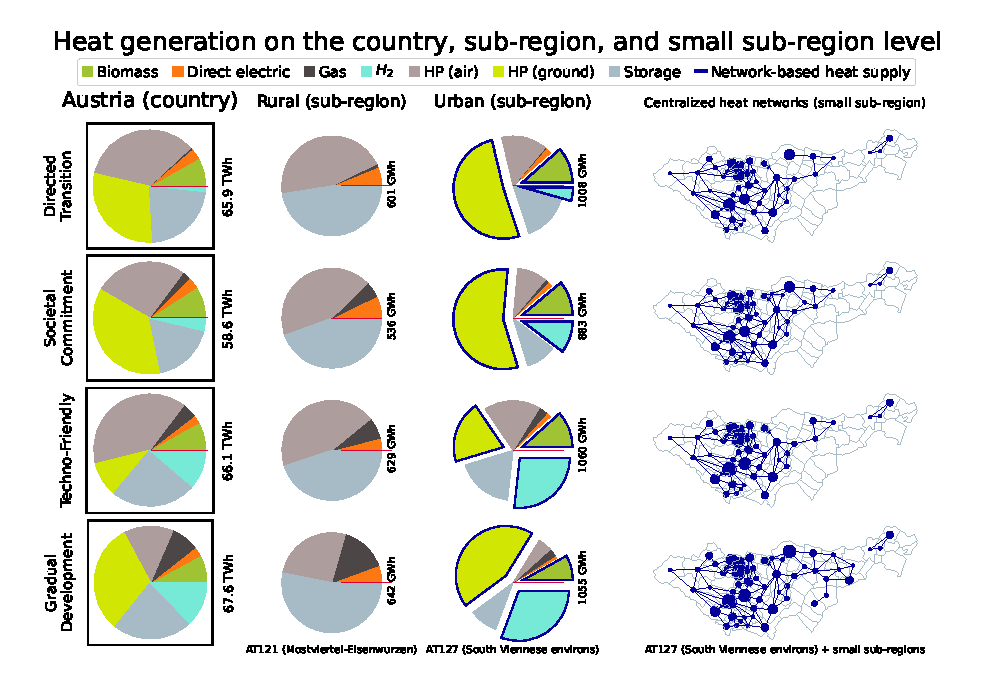
\includegraphics[width=1\linewidth]{figures/4_Results/Spatial_results.eps}
	\caption{Low temperature heat technology generation on different spatial granularity levels for the four different storylines. left: heat technology generation mix on the country level. middle: comparison of technologies supplying the low temperature heat demand in a rural and urban sub-region. right: Centralized heat network topology (size of the points represent the amount of local heat demand supplied by the centralized heat network)}
	\label{fig:res1}
\end{sidewaysfigure}
\newpage
\subsection{Austrian sub-regions with high potentials for centralized low temperature heat supply resulting from aiming the decarbonization}\label{res:3}
As already indicated by Figure \ref{fig:res1}, the results show that there are only a limited number of sub-regions in Austria that have sufficient population and thus heat density to allowing centralized heat supply. Figure \ref{fig:res2} shows a heatmap for centralized heat supply in Austria 2050. Thereby, the spatial granularity corresponds to sub-regions or the NUTS3 level respectively. The corresponding six sub-regions are supplied by the heat networks independent of the storylines. However, the individual quantities of centralized heat supply per sub-region do differ between the storylines (see also exemplarily the heat technology generation mix of the sub-region AT127 in the middle of Figure \ref{fig:res1}). In addition, two comments are essential in this context. Firstly, that Figure \ref{fig:res2} only shows the quantity of centralized heat supply per sub-region. At the same time, heat generation technologies that are not fixed to a central heat distribution network also supply some parts of the heat demand there (see again exemplarily the heat technology generation mix of the sub-region AT127 in the middle of Figure \ref{fig:res1}). Therefore, in those sub-regions in Figure \ref{fig:res2} that are completely white and thus do not have a supply by a centralized heat network, it is shown by the results that the heat demand there is completely covered by technologies that do not require a heat network infrastructure. And secondly, that as expected, the coloured areas are those with the highest population density. This varies between \SI{229}{persons \per \kilo\metre^2} (AT323 - Salzburg and sourroundings) and \SI{5124}{persons \per \kilo\metre^2} (AT130 - Vienna). As indicated in Figure \ref{fig:res2} (orange box), in the following section, the marked sub-regions are further spatially dissaggregated. Subsequently, their heat network topology is analyzed. 

\begin{sidewaysfigure}
	\centering
	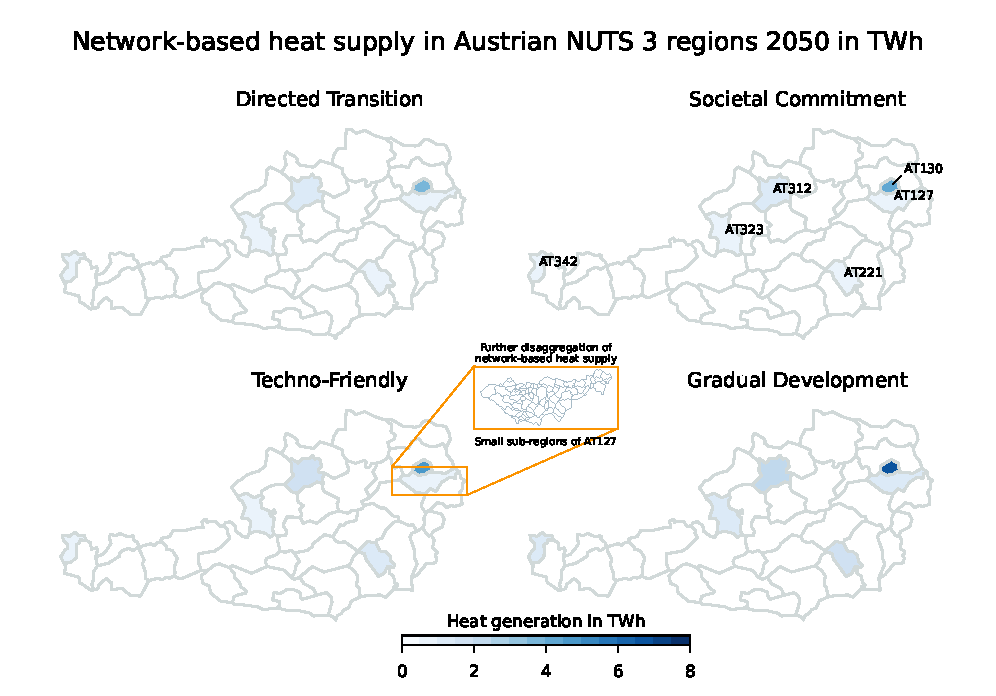
\includegraphics[width=1\linewidth]{figures/4_Results/Heatmap.eps}
	\caption{Centralized low temperature heat supply in Austria 2050. Six sub-regions provide sufficient values of population density to supply parts of the low temperature heat demand by heat networks. The remaining heat demand is supplied by on-site heat technology options. }
	\label{fig:res2}
\end{sidewaysfigure}

\newpage
\subsection{Low temperature heat network topology on the small sub-region level}\label{res:4}
This section analyzes the heat network topology of those regions, that provide sufficient characteristic in terms of population density for centralized heat supply. Figure \ref{fig:res3} shows the boxplot of the benchmark indicator value for the sub-region AT127 (including all small sub-regions). The number of small sub-regions supplied by the centralized heat network is plotted on the horizontal axis. Note that this number decreases from left to right. It becomes visible that by removing small sub-regions, namely iteratively those with the smallest indicator value, the mean indicator value of the entire remaining heat network increases. In addition, the maximum value of the indicator also increases from under 1.64 to over 7.16. In the present example, the number of small sub-regions supplied by the centralized heat network decreases from \SI{75}{} to \SI{47}{} (\SI{-37.3}{\%}). The iteratively reduction of supplied small sub-regions does not necessarily result in a contigous graph. For example, three small sub-regions form a subgraph that is separate from the other network (see upper right in the green box in Figure \ref{fig:res3}).\newline

The results discussed above suggest that reducing the number of small sub-regions supplied by the centralized heat network increase the indicator value and thus the efficiency of the heat network topology. Simultaneously, this also increases the heat density of the supply area. In the following subsection, the obtained heat density values of the heat networks are compared with existing values and today's minimum required values for centralized heat networks.

\begin{sidewaysfigure}
	\centering
	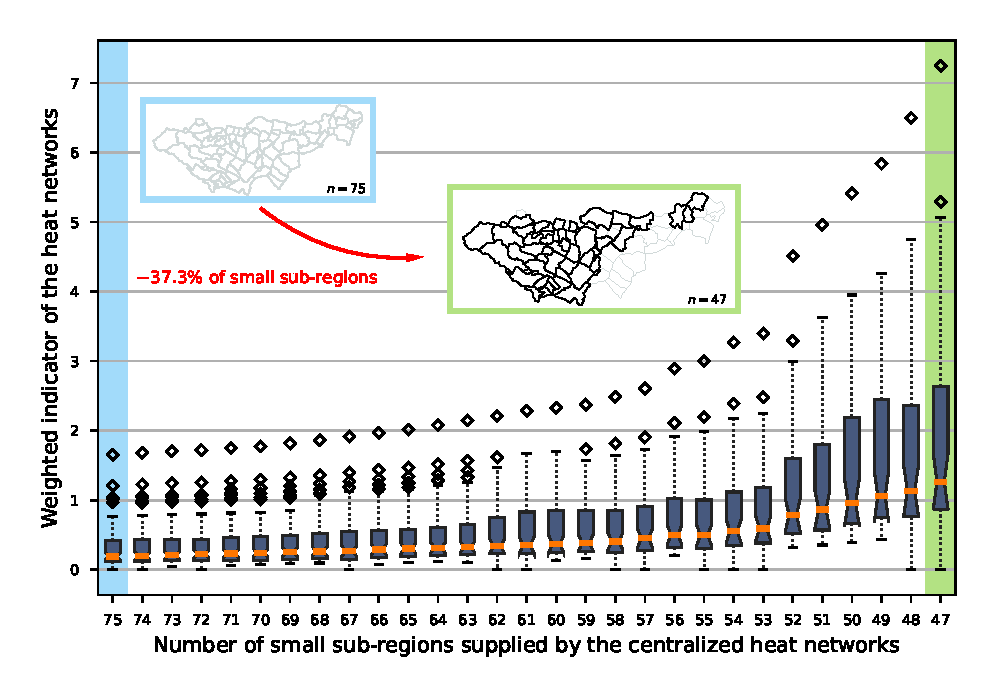
\includegraphics[width=1\linewidth]{figures/4_Results/boxplot.eps}
	\caption{Weighted indicator value of the low temperature heat network at the sub-region AT127 (South Viennese environs) for different numbers of areas supplied by the centralized heat networks.}
	\label{fig:res3}
\end{sidewaysfigure}
\newpage
\subsection{Comparison of existing and future projections of low temperature heat networks using heat and population density}\label{res:5}
This section synthesizes the results in the context of heat density values of centralized heat networks and compares the obtained future projections of sustainable centralized heat supply with current minimum required heat density standards of heat networks. Figure \ref{fig:res4} shows the heat density of low temperature heat networks for different the different proposed downscaling techniques and the four different storylines. The population density is shown on the horizontal axis. The black triangles mark the minimum required heat density for today's centralized heating networks at a connection rate of \SI{90}{\%} in Austria.\footnote{See in this context for example \url{http://www.austrian-heatmap.gv.at/karte/}.} The circles ($\bullet$) mark the default downscaling with only population as criterion. Therefore, the heat density of the sub-regions increases linearly with the population density (see also the zoomed out area in the left subfigure with population density $\leq 150 \frac{persons}{km^2}$). The diamonds ($\blacklozenge$) mark the heat density values obtained by Algorithm 1 (and thus without supply area reduction). As a result, the heat density per sub-region increases (see the zoomed out area in the middle subfigure with population density $\leq 500 \frac{persons}{km^2}$). The stars ($\bigstar$) mark the heat density resulting by Algorithm 2. In order to highlight the effects of the different downscaling techniques, the differences of the resulting heat densities to today's minimum required values is shown for a sub-region by the three green bars for the \textit{Techno-Friendly} storyline. As the comparison of the green bars shows, the difference is again significantly reduced by applying Algorithm 2.

\begin{sidewaysfigure}
	\centering
	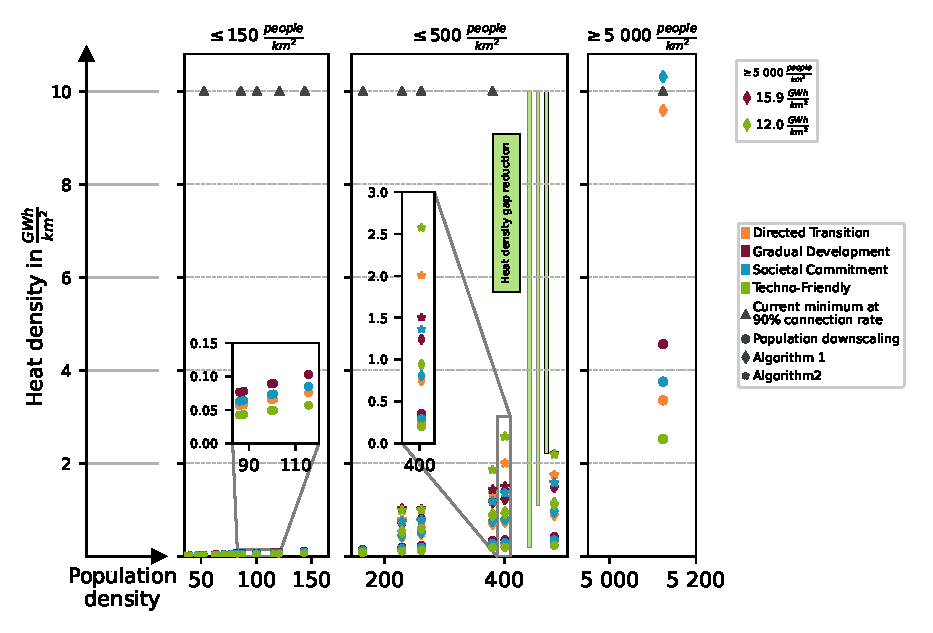
\includegraphics[width=1\linewidth]{figures/4_Results/Heat_density_gap.eps}
	\caption{Heat densities for different population densities, decarbonization storylines, and downscaling techniques. Reducing significantly the gap between today's minimum required heat density (\SI{10}{\frac{GWh}{km^2}} at a connection rate of \SI{90}{\%}) by Algorithm 2 in comparison with default population-based downscaling.}
	\label{fig:res4}
\end{sidewaysfigure}

\section{Conclusions and recommendations}\label{conclusions}
\added{The} sustainable energy transition requires methods to bridge the gap between global decarbonization pathways and the \replaced{corresponding}{resulting necessary} measures at local levels. This work emphasizes the development of different downscaling \replaced{techniques}{algorithms}, which we apply to the European heating sector under several \replaced{scenarios}{storylines} in line with the Paris Agreement \added{and its remaining CO\textsubscript{2} budget}. \added{We use the cost-effective European heat supply from the aggregate model GENeSYS-MOD to analyze results at the community level in Austria. The remaining European CO\textsubscript{2} budget (and related CO\textsubscript{2} prices) in line with the 1.5°C climate target is considered by the GENeSYS-MOD results. The downscaling includes the technology-specific infrastructure requirements for the highly efficient usage of heat sources in district heating}.\vspace{0.3cm}

\added{We found that the cost-effective heat supply at the European and national level in 2050 implies that district heating covers parts of the heat demand in four of the thirty-five sub-regions in Austria. Furthermore, the results demonstrate that district heating continues to be picking cherries from beneficial areas (i.e., densely populated with high heat densities) as only some communities of the four mentioned areas are supplied by district heating. Nevertheless, not all district heating networks and supply areas in 2050 reach the heat density required for economic and technical efficiency from today’s techno-economic perspective and industry benchmarks. This heat density gap (mainly driven by a significant reduction of heat demands by building renovation measures) poses a challenge for district heating but can be reduced by the optimal allocation of large-scale heat pump (air) generation into district heating.}\vspace{0.3cm}

\added{We anticipate our work as a starting point for discussing the role of district heating enabling large-scale, highly efficient, and local integration of renewable heat sources such as geothermal, synthetic gas, hydrogen, and waste in sustainable energy systems with decreasing heat demands. Further research should follow on how obtained district heating networks and their heat densities (incl. the generation of large-scale heat pump (air) units) could be returned into more aggregate models, such as GENeSYS-MOD, in the sense of a feedback loop. That allows refining assumptions in the large-scale models, which in turn will increase the plausibility and realism of pathways at the European level.}



\section*{Declaration of interests}
None.
\section*{Declaration of Competing Interest}
The authors report no declarations of interest.
\section*{Acknowledgments}
This project has received funding from the European Union's Horizon 2020 Research and Innovation Programme under Grant Agreement No. 835896. Part of the research was developed in the Young Scientists Summer Program (YSSP) at the International Institute for Applied Systems Analysis(IIASA), Laxenburg (Austria). The authors acknowledge TU Wien Bibliothek for financial support through its Open Access Funding Programme.

\bibliography{mybibfile}
\appendix
\setcounter{table}{0}
\setcounter{figure}{0}

\section{Current Austrian heat market}\label{appendixC}
\added{Table \ref{tab:numbers} provides an overview of the Austrian heat market in 2017. Particularly, the proportion per heat source/generation technology on the total heat demand for space heating and hot water is shown. Note that the absolute number of households supplied by heat pumps and solarthermal is in total 294,075 (see row 6 in the table). According to \cite{statisitik2016}, the total heat production from district heating was around} \SI{24}{TWh} \added{in 2016. Thereby, the share of renewable energy was 45\%. Besides, the share of waste sources was 9\%.}  

\definecolor{Gray}{gray}{0.95}
\begin{table}[h]
	\centering
	\resizebox{1\textwidth}{!}{% use resizebox with textwidth
		\renewcommand{\arraystretch}{1.1}
		\begin{tabular}{lcc}
			\toprule 
			& Proportion in \% & Abs. number\\\cmidrule(rl){2-2}\cmidrule(rl){3-3}
			Heat source/technology& on space and hot water demand & of households supplied\\\hline
			Biomass & 28.3 & 725,439\\
			Natural gas & 26.5 & 913,448\\
			Oil & 17.2 & 626,109\\
			District heating & 14.6 & 1,112,734\\
			Direct electric & 8.2 & 210,648\\
			Heat pumps & 3.0 & \multirow{2}{*}{294,075}\\
			Solarthermal & 1.9 & \\
			Coal & 0.4 & 7,640\\
			\bottomrule
	\end{tabular}}
	\caption{\added{Proportion of heat sources/generation technologies on the total heat demand (space and hot water) and absolute number of households supplied for Austria in 2017. Source: \cite{oesterreichsenergie}.}}
	\label{tab:numbers}
\end{table}

\section{Illustration of the benchmark indicator value}\label{appendixB}
Figure \ref{fig:app:method} shows an illustrative example of the iterative downscaling algorithm (Algorithm 2). It shows two different conditions of a simple graph. In the first condition ($i$), the network topology consists of four nodes (A-D) and four lines. It is shown in the subfigure in the top left. The table below (bottom left) shows the amount of \replaced{district heating}{centralized} and on-site heat supply as well as the indicator value for each node. Note that the numbers are only for illustration. Node A has the lowest indicator value (see marker [1] in the left table) and, therefore, its amount of \replaced{district heating}{centralized heat supply} (marker [2]) is reallocated to the remaining nodes of the network (marker [3]). This process increases the on-site heat supply accordingly at node A as this node is not connected to the network in condition $i+1$ and increases the amount of \replaced{district heating}{centralized heat supply} at nodes B-D (see the larger nodes in the top right subfigure). The heat demand of node A in condition $i+1$ is covered only by on-site heat supply. Node A is removed from the graph and thus disconnected from the network.

\begin{figure}[h]
	\centering
	\includegraphics[width=1\linewidth]{figures/_appendix/Method_appendix.pdf}
	\caption{Illustrative example of Algorithm 2 showing a simple graph with four nodes in two different conditions. The node with the lowest indicator value in condition $i$ (node A) is removed from the graph (markers [1]-[3] in the table at the bottom left). The amount of \replaced{district heating}{centralized heat supply} from node A is reallocated to the remaining nodes B-D (see table at the bottom right).}
	\label{fig:app:method}
\end{figure}

\section{Data and further empirical settings}\label{appendixA}
\begin{table}[h]
	\centering
	\scalebox{0.85}{
		\renewcommand{\arraystretch}{1.35}
		\begin{tabular}{lccc}
			\toprule 
			& Description & Data availability & Data source\\\hline
			GENeSYS-MOD v2.0 & Heat generation by source & \cite{explorer} & \cite{loffler2017designing}\\
			Austrian population density & in 2019 & \multicolumn{2}{c}{\href{https://www.statistik.at/web_de/statistiken/index.html}{\textit{Statistik Austria}}}\\
			Austrian population & in 2050 & \multicolumn{2}{c}{\href{https://ec.europa.eu/eurostat/databrowser/view/tps00003/default/table?lang=en}{\textit{Eurostat}}}\\
			\bottomrule
	\end{tabular}}
	\caption{Empirical data settings}
	\label{tab:a2}
\end{table}

\section{Heat density for varying allocation of heat pump generation into district heating}\label{Appendix:D}
\added{Figure \ref{fig:sens} shows the heat density of the district heating network in Graz (AT221) in the \textit{Directed Transition} scenario. On the x-axis, the amount of district heating is shown. District heating in the \textit{Directed Transition} scenario includes synthetic gas and waste only. The corresponding heat density is indicated by the black circle (top). The range between the two dotted lines marks the heat generation by heat pump (air) units. The left dashed line indicates heat pump (air) generation if used exclusively on-site (i.e., small-scale heat pump (air) units). Similarly, the right dashed line indicates heat pump (air) generation if used exclusively in district heating (i.e., large-scale heat pump (air) units). Each point between the two dashed lines corresponds to an individual split between small- and large-scale heat pump (air) units. The maximum heat density of} \SI{10.9}{GWh \per km^2} \added{is reached by a share of two-thirds of large-scale heat pump (air) units feeding into district heating while one-third is on-site.}

\begin{figure}[h]
	\centering
	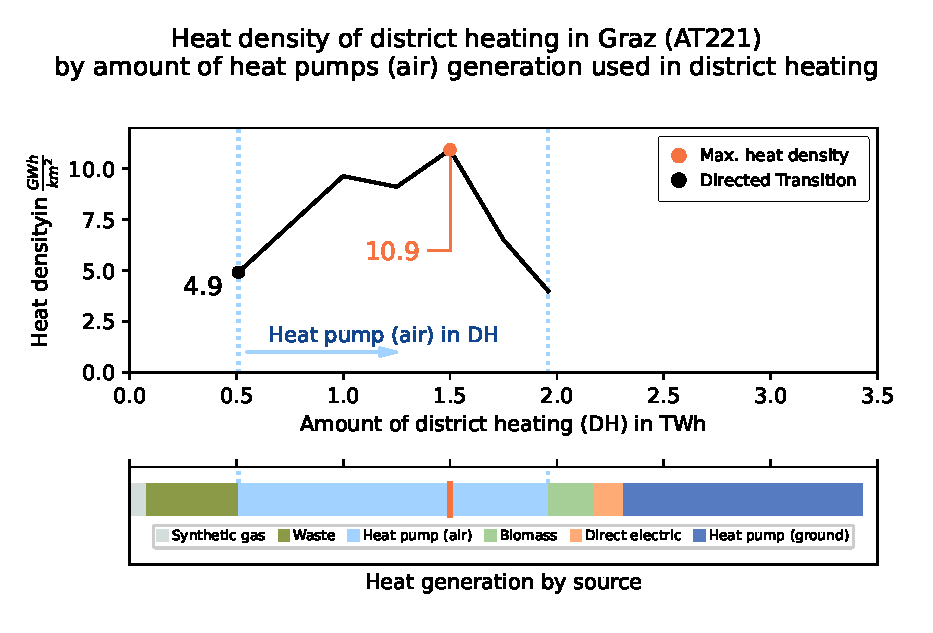
\includegraphics[width=1\linewidth]{Figures/4_Results/Sensitivity_Analysis/Sen_District_heating.eps}
	\caption{\added{Heat density of the district heating network in Graz (AT221) in the \textit{Directed Transition} scenario (black circle) and for varying allocation of heat pump (air) generation into district heating (black line). The maximum heat density of} \SI{10.9}{GWh \per km^2} \added{is reached by a share of two-thirds of heat pump (air) generation feeding into district heating.}}
	\label{fig:sens}
\end{figure}

\end{document}